\item \begin{theorem}{(233, 236, 240)} Graph:\begin{itemize}
        \item Adjacency multilists:每個節點儲存$v_i$,$v_j$,$link\_for\_v_i$指向$v_i$下一個相鄰的點所在的節點,$link\_for\_v_j$指向$v_j$下一個相鄰的點所在的節點。% 例子:\ref{img:adj_multilists}。
        \item 無向圖只有tree edge和back edge。判斷無向圖back edge(cycle):兩個點都gray,但是不為父子節點。
        \begin{table}[H]
            \centering
            \begin{tabular}{|c|c|c|}
                \hline
                Operation & Adjacency matrix & Adjacency lists \\
                \Xhline{2\arrayrulewidth}
                Lots of vertices & & $\surd$ \\
                \hline
                \makecell{\# of edges or \\if it's connected, etc.} & & $\surd \ (O(|\V| + |\E|))$ \\
                \hline
            \end{tabular}
        \end{table}
        \begin{table}[H]
            \centering
            \begin{tabular}{|c|c|c|}
                \hline
                Data structure & DFS & BFS \\
                \Xhline{2\arrayrulewidth}
                Adjacency matrix & \multicolumn{2}{c|}{$O(|\V|^2)$} \\
                \hline
                Adjacency lists & \multicolumn{2}{c|}{$O(|\V| + |\E|)$} \\
                \hline
            \end{tabular}
        \end{table}
        \begin{figure}[H]
            \centering
            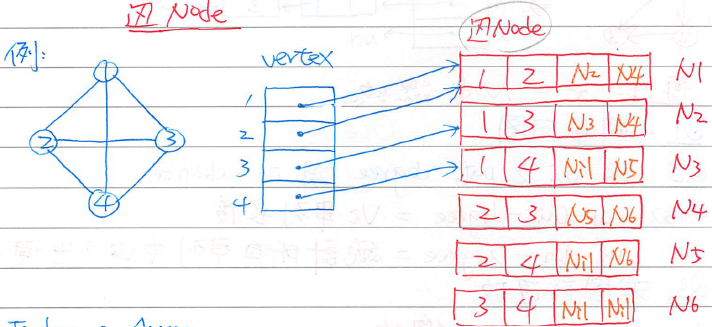
\includegraphics[scale=0.8]{img/adj_multilists.png}
            \caption{Example for adjacency multilists.}
            \label{img:adj_multilists}
        \end{figure}
    \end{itemize}
\end{theorem}

\item \begin{theorem}{(257)} 尋找articulation point:\begin{itemize}
        \item $dfn$為DFS number。
        \item \begin{equation}
            low(v) = \begin{cases}
                dfn(v) \\
                \min\{low(u) | u \ \text{is child of} \ v\} \\
                dfn(u), u \ \text{is descendant of} \ v\text{, which is reachable by a back edge}
            \end{cases} , \forall v \in G
        \end{equation}
        \item 若root有$\ge 2$子節點,則root為articulation point;非root節點$u$,若$\exists v$為$u$子節點,且$low(v) \ge dfn(u)$,則$u$為articulation point。
    \end{itemize}
\end{theorem}
